\documentclass[a4paper,twoside]{article}

\usepackage{epsfig}
\usepackage{subcaption}
\usepackage{calc}
\usepackage{amssymb}
\usepackage{amstext}
\usepackage{amsmath}
\usepackage{amsthm}
\usepackage{multicol}
\usepackage{pslatex}
\usepackage{apalike}
\usepackage{csquotes}
\usepackage[hidelinks]{hyperref}
\usepackage[capitalize]{cleveref}
\Crefname{figure}{Fig.}{Figs.}
\Crefname{section}{Sec.}{Secs.}
\Crefname{table}{Tab.}{Tabs.}
\Crefname{equation}{Eq.}{Eqs.}
\usepackage{numprint}
\usepackage{SCITEPRESS} 

\usepackage{microtype} %

\usepackage{calc}
\usepackage{tikz}
\usetikzlibrary{calc,positioning,spy,shapes}


\tikzset{thick/.style = {line width = 1.0pt}}

\newlength{\pfull}  \setlength{\pfull}  {2mm}
\newlength{\phalf}  \setlength{\phalf}  {0.5\pfull}

\newlength{\lwffp}   \setlength{\lwffp}   {0.5000\dimexpr(\linewidth-1.0\pfull)}
\newlength{\lwfffp}  \setlength{\lwfffp}  {0.3333\dimexpr(\linewidth-2.0\pfull)}
\newlength{\lwffffp} \setlength{\lwffffp} {0.2500\dimexpr(\linewidth-3.0\pfull)}
\newlength{\lwfffffp}\setlength{\lwfffffp}{0.2000\dimexpr(\linewidth-4.0\pfull)}

\newlength{\twffp}   \setlength{\twffp}   {0.5000\dimexpr(\textwidth-1.0\pfull)}
\newlength{\twfffp}  \setlength{\twfffp}  {0.3333\dimexpr(\textwidth-2.0\pfull)}
\newlength{\twffffp} \setlength{\twffffp} {0.2500\dimexpr(\textwidth-3.0\pfull)}
\newlength{\twfffffp}\setlength{\twfffffp}{0.2000\dimexpr(\textwidth-4.0\pfull)}

\tikzstyle{labelStyle} = [ shape = rectangle, font = \scriptsize, text depth = 0, fill = white, inner sep = 4pt ]
\tikzstyle{labelN}  = [ labelStyle, anchor = north ]
\tikzstyle{labelNW} = [ labelStyle, anchor = north west ]
\tikzstyle{labelNE} = [ labelStyle, anchor = north east ]
\tikzstyle{labelS}  = [ labelStyle, anchor = south ]
\tikzstyle{labelSW} = [ labelStyle, anchor = south west ]
\tikzstyle{labelSE} = [ labelStyle, anchor = south east ]

\tikzstyle{figRC} = [shape = rectangle, rounded corners = 2mm, clip] % figure with Rounded Corners
\tikzstyle{spyRC} = [shape = rectangle, rounded corners = 2mm, %
    darkgray, connect spies, every spy on node/.append style = {thick}] % spy with Rounded Corners
\tikzstyle{figNS} = [inner sep = 0pt, outer sep = 0pt] % figure with No Separators
 %

\usepackage{flushend}
\usepackage[switch]{lineno}
\usepackage{xspace}
\usepackage{siunitx}

\usepackage{tikz}
\usetikzlibrary{calc,positioning,spy}

\usepackage{booktabs}

\usepackage{float}
\newfloat{lstfloat}{htbp}{lop}
\floatname{lstfloat}{Listing}

\usepackage[nolist]{acronym}


\usepackage{listings} 
\usepackage{accsupp}


% This ensures numbers are not copied, but leading spaces are copied, as taken from
% http://tex.stackexchange.com/a/30310

\newcommand{\noncopynumber}[1]{%
    \BeginAccSupp{method=escape,ActualText={}}%
    #1%
    \EndAccSupp{}%
}

\makeatletter
\def\lst@outputspace{{\ifx\lst@bkgcolor\empty\color{white}\else\lst@bkgcolor\fi\lst@visiblespace}}
\makeatother


\definecolor{msvc_keyword}   {HTML}{0000FF} 
\definecolor{msvc_comment}   {HTML}{008000} 
\definecolor{msvc_background}{HTML}{eff0f1} 
\definecolor{msvc_frame}     {HTML}{000000}
\definecolor{msvc_linenumber}{HTML}{808080}
\definecolor{msvc_string}    {HTML}{000000}

\definecolor{msvc_directives}{HTML}{808080}
\definecolor{msvc_operators} {HTML}{000000}
\definecolor{msvc_stl}       {HTML}{000000}


\lstdefinelanguage{TypeScript}
{
    keywords        = {break, case, catch, continue, debugger, default, delete, do, else, finally, for, function, if, in, instanceof, new, return, switch, throw, try, typeof, var, void, while, with, super, class, constructor},
    morecomment     = [l]{//},
    morecomment     = [s]{/*}{*/},
    morestring      = [b]',
    morestring      = [b]", 
    keywordstyle    = \color{blue}\bfseries,
    identifierstyle = \color{black},
    commentstyle    = \color{teal}\ttfamily,
    stringstyle     = \color{red}\ttfamily,
    sensitive       = true,
    style           = TypeScript
}


\lstdefinestyle{TypeScript}
{
    basicstyle       = 
\linespread{0.85}\ttfamily
\lst@ifdisplaystyle\scriptsize\fi %inline code should have normal font size
%
,   backgroundcolor  = \color{msvc_background}
,   rulecolor        = \color{msvc_frame}
,   keywordstyle     = \lst@ifdisplaystyle\color{msvc_keyword}\fi
,   commentstyle     = \lst@ifdisplaystyle\color{msvc_comment}\fi
,   stringstyle      = \lst@ifdisplaystyle\color{msvc_string}\fi
,   showstringspaces = false
,   numberbychapter  = true
,   numbersep        =  8pt
,   showlines        = true
,   tabsize          =  2          
,   numbers          = left
,   numberstyle      = \tiny\color{msvc_linenumber}\noncopynumber
,   framesep         =  4pt
,   xleftmargin      = \parindent
,   xleftmargin      = 16pt
,   framexleftmargin = 16pt
,   abovecaptionskip = \medskipamount
,   stepnumber       = 1
,   columns          = flexible
,   keepspaces       = true
,	keywords         = [2]{ prototype, this }
,	keywordstyle     = [2]\lst@ifdisplaystyle\color{msvc_stl}\fi
,   morekeywords     = [1]{ noexcept }
,	literate         = *
{[}{{\lst@ifdisplaystyle\color{msvc_operators}\fi{[}}}{1}
{]}{{\lst@ifdisplaystyle\color{msvc_operators}\fi{]}}}{1}
}


\makeatletter
\DeclareRobustCommand\onedot{\futurelet\@let@token\@onedot}
\def\@onedot{\ifx\@let@token.\else.\null\fi\xspace}
\def\etal{et~al\onedot\xspace}
\def\ie{i.e.,\xspace}
\def\eg{e.g.,\xspace}
\makeatother

\begin{document}
\title{Visualization of Knowledge Distribution across Development Teams using 2.5D Semantic Software Maps}

\author{
\authorname{Daniel Atzberger,
    Tim Cech,
    Adrian Jobst,\\
    Willy Scheibel\orcidAuthor{0000-0002-7885-9857},
    Daniel Limberger\orcidAuthor{0000-0002-9111-4809},
    Matthias Trapp\orcidAuthor{0000-0003-3861-5759},
    and Jürgen Döllner}
    \affiliation{Hasso Plattner Institute, Digital Engineering Faculty, University of Potsdam, Germany}
    \email{\{daniel.atzberger,
    tim.cech,
    willy.scheibel,
    daniel.limberger,
    juergen.doellner\}@hpi.uni-potsdam.de
    \\
    \{adrian.jobst\}@student.hpi.uni-potsdam.de
}
}

\keywords{Topic Modeling, Software Visualization, Source Code Mining}

\abstract{
In order to detect software risks at an early stage, various software visualization techniques have been developed for monitoring the structure, behaviour, or the underlying development process of software.
One of greatest risks for any IT organization consists in an inappropriate distribution of knowledge among its developers, as a projects' success mainly depends on assigning tasks to developers with the required skills and expertise.
In this work, we address this problem by proposing a novel Visual Analytics framework for mining and visualizing the expertise of developers based on their source code activities.
Under the assumption that a developer's knowledge about code is represented directly through comments and the choice of identifier names, we generate a 2D layout using Latent Dirichlet Allocation together with Multidimensional Scaling on the commit history, thus displaying the semantic relatedness between developers.
In order to capture a developer's expertise in a concept, we utilize Labeled LDA trained on a corpus of Open Source projects.
By mapping aspects related to skills onto the visual variables of 3D glyphs, we generate a 2.5D Visualization, we call \textit{KnowhowMap}.
We exemplify this approach with an interactive prototype that enables users to analyze the distribution of skills and expertise in an explorative way.
}

\onecolumn \maketitle \normalsize \setcounter{footnote}{0} \vfill

\section{\uppercase{Introduction}}
\label{KM:Sec:Introduction}

\paragraph{Visual Analytics for Software Data}
\label{KM:SubSec:Context}

The complexity of modern software development projects requires careful coordination of all development activities, which are usually managed using various interactive tools with visualization capabilities.
Therefore during the entire development process, data from heterogeneous categories is generated and stored in respective software repositories.
For example, changes in the source code made by the developers are represented in a \ac{VCS}, the progress of development tasks is tracked within an issue tracking system, defects are reported, assigned and managed in a bug tracking system, and discussions on selected topics are conducted in chat forums by the developers.
These rich sources of data motivate the use of machine learning techniques when mining software repositories~\cite{bird2015art}.

Complementary to the analysis of software data using machine learning techniques, Software Visualization techniques can be applied to communicate various aspects of the structure or behaviour of a software system using graphical representations.
Often, the analysis and visualization go hand in hand, therefore being an example for the broader field of Visual Analytics~\cite{keim2008visual}.

\begin{figure*}[t] %
    \begin{tikzpicture}[figNS, spy using outlines = {style = spyRC, magnification = 1.8, size = 24mm}]
        \node[figRC, anchor = center](fig0) at (0,0)
            {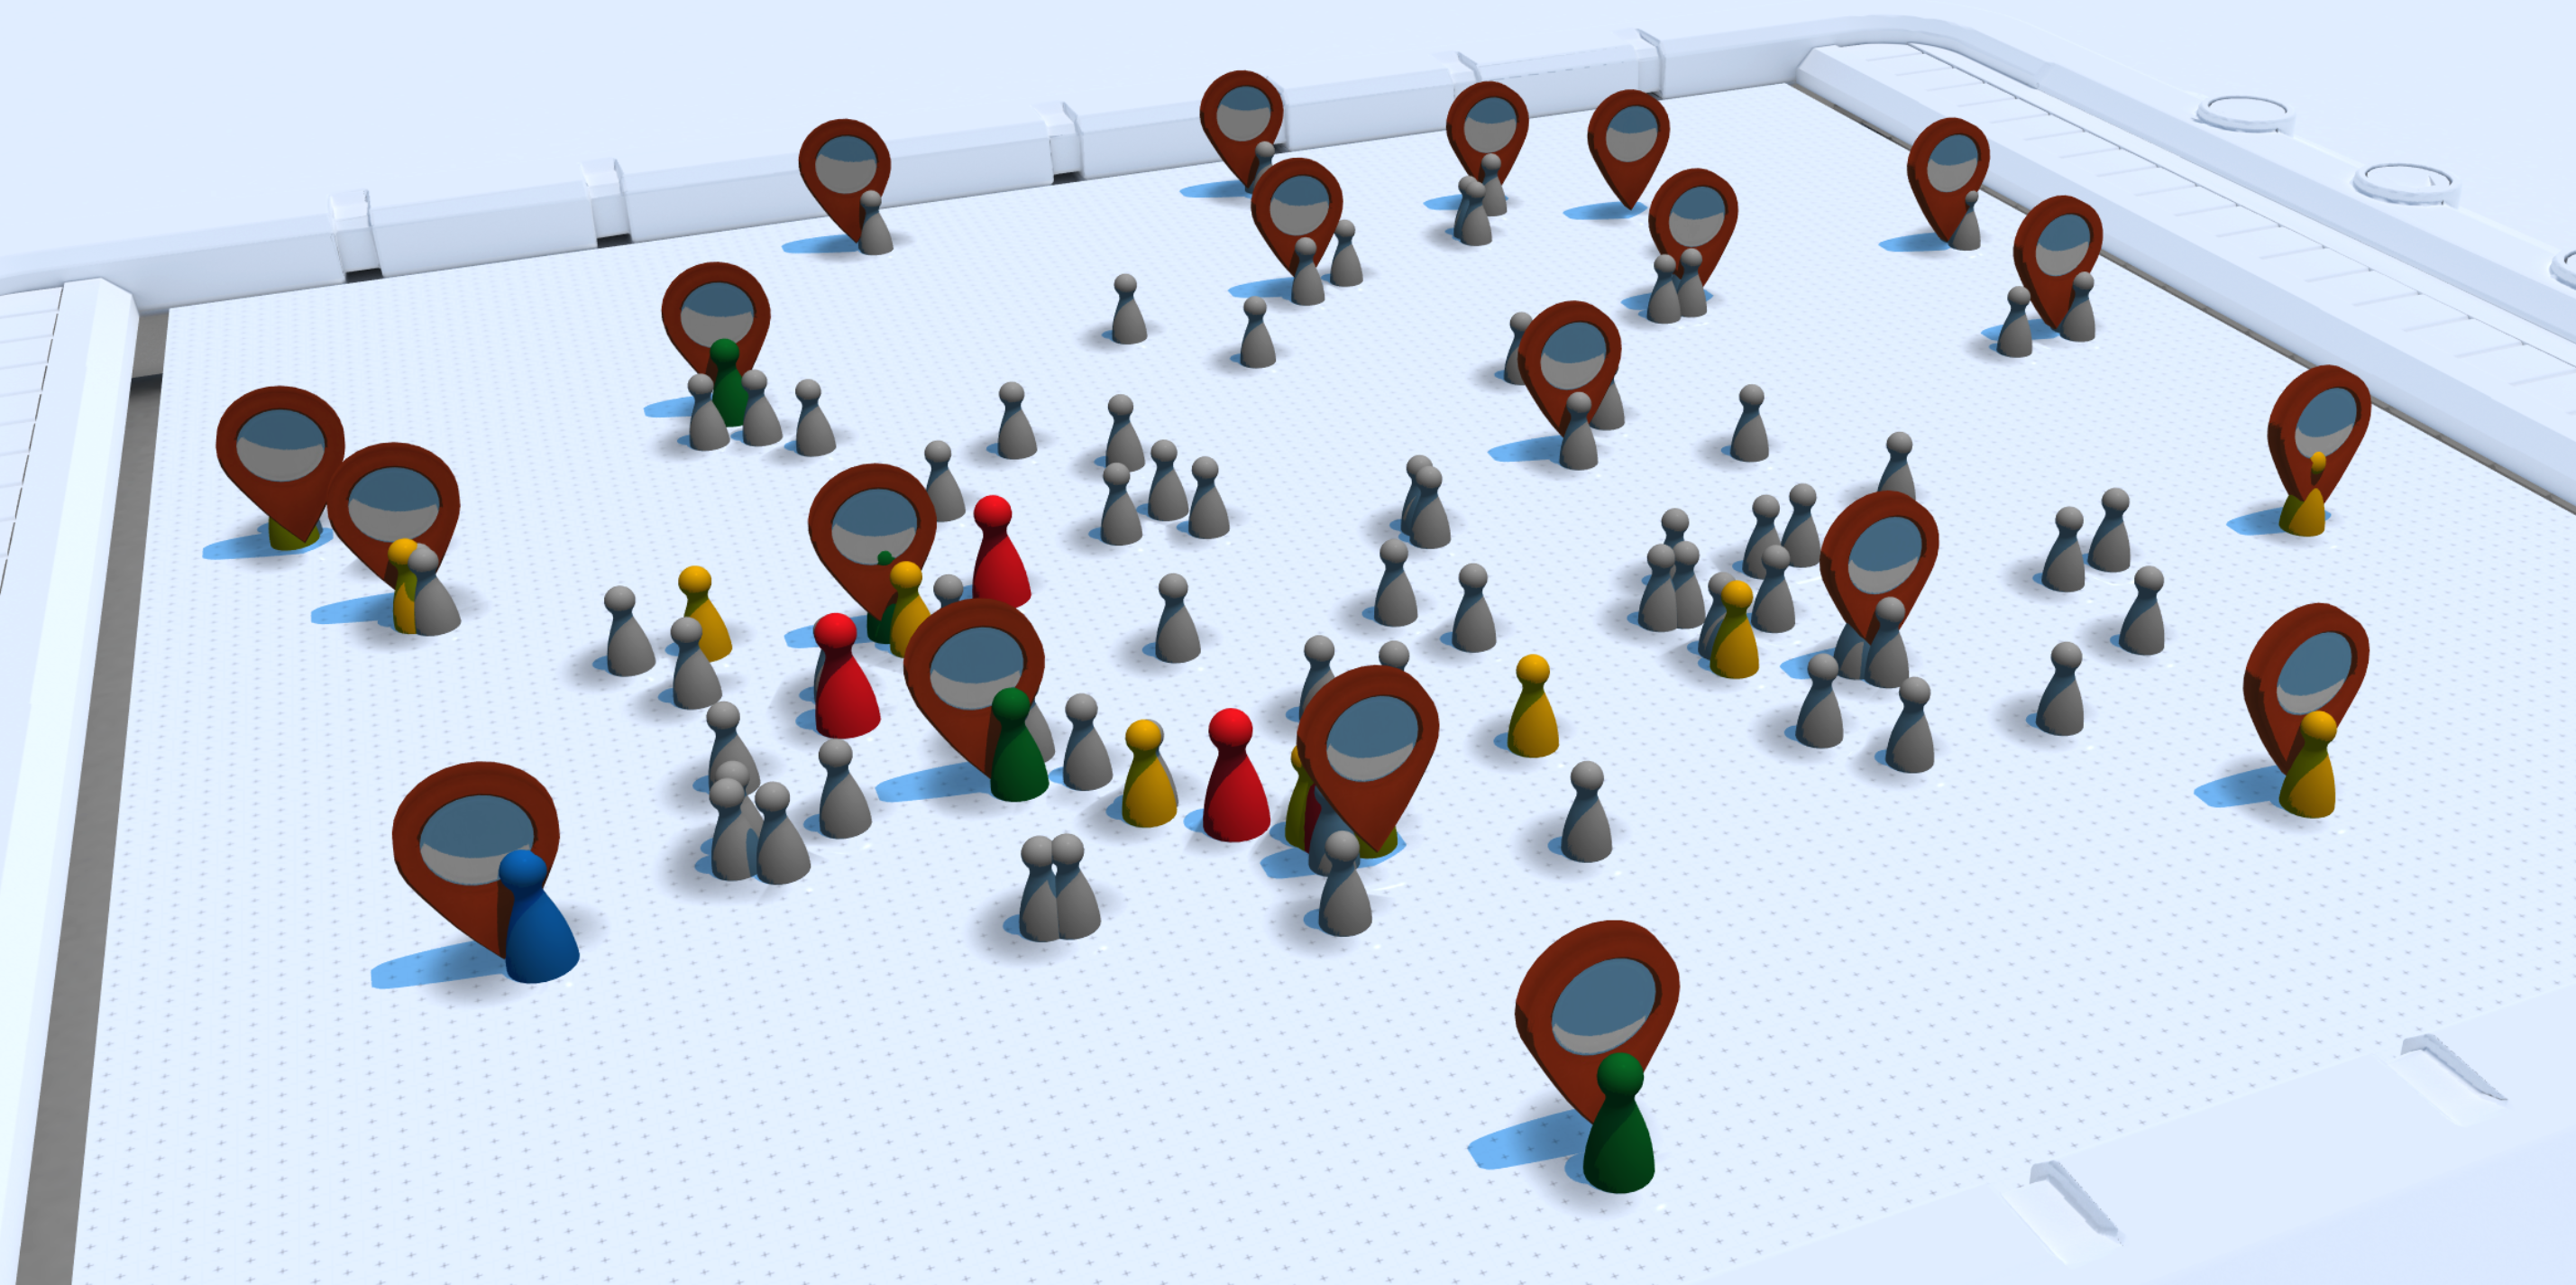
\includegraphics[width = \textwidth, trim = 0 0 0 0, clip]{knowhowmap-bitcoin-v3-trimmed_2.png}};
    \end{tikzpicture}
    \caption{\textit{KnowhowMap} for the \textit{Bitcoin Core} project(\href{https://github.com/bitcoin/bitcoin}{github.com/bitcoin/bitcoin}) based on 2000 commits. Each developer is displayed as a pawn figure, whose height displays its expertise level in the concept \textit{Cryptocurrency}. The pointers display latent source code topics.}
    \label{KM:Fig:BitcoinTeaser}
\end{figure*}

Examples for Software Visualizations supporting program comprehension tasks or risk monitoring include treemaps based on the folder structure of source code projects, where additional quantitative data about a software's quality or complexity is mapped to visual variables~\cite{Bohnet2011Monitoring,limberger2019-softwaremap,scheibel2020-treemaptaxonomy}, circular bundle views for displaying dependencies between source code files~\cite{Truemper2012CBV}, trace visualization techniques~\cite{truemper2010trace} or software landscapes displaying the semantic structure that is captured from investigating the use of natural language in comments and identifier names using topic models~\cite{kuhn2008consistentlayout,atzberger2021softwareforest,atzberger2021-softwaregalaxy}.

\paragraph{Problem Statement}
\label{KM:SubSec:Challenges}
According to Sommerville~\cite{sommerville2016softwareengineering} \enquote{The people working in a software organization are its greatest assets}, therefore it is of fundamental importance for any IT organization to keep track of the distribution of knowledge across its developer staff.
The existing approaches of analyzing knowledge of developers all focus on specific aspects and do thus not allow a user, \eg a project manager, to investigate the distribution of knowledge in an explorative way.
An interactive visualization technique should address the following aspects:

\begin{enumerate}
    \item \textbf{Similarity between developers}, given as a numerical value between 0 and 1, which is the basis for all questions on the distribution of skills.
    \item \textbf{Visualization of categorical attributes}, as properties, such as the location or the team membership are of discrete nature.
    \item \textbf{Visualization of numerical attributes}, as the level of skills in a concept or technology can be measured on a numerical scale.
\end{enumerate}

\paragraph{Approach and Contributions}
\label{KM:SubSec:Approach}

In this work, we propose a concept for mining and visualizing the distribution of knowledge across software organizations on the basis of their activities stored in the \ac{VCS}.
By applying \ac{LDA}, a probabilistic topic model, on the commit histories of developers, we can compare developers on a semantic level.
A subsequent application of dimension reduction techniques generates a 2D layout for presenting the \enquote{similarity} between the developers.
Using a novel concept-location approach based on \ac{LLDA}, we assign an expert level to each developer with respect to  general concepts, \eg \textit{Machine Learning} or \textit{Blockchain}.
The so-generated data is then mapped onto the visual variables of 3D glyphs, that leads a visualization, we call \textit{KnowhowMap}.
An example for a \textit{KnowhowMap} for the \textit{Bitcoin} project is shown in \Cref{KM:Fig:BitcoinTeaser}.
To summarize, we make the following contributions
\begin{enumerate}
\item We present an approach for mining the expertise of developers in general concepts using \ac{LLDA}.
\item We present a 2.5D visualization technique, whose layout reflects the semantic relatedness between developers and whose glyphs can be used to display various data related to developer data.
\end{enumerate}

\noindent The remainder of this work is structured as follows:
\Cref{KM:Sec:Background} describes preliminaries on data sets and concept.
\Cref{KM:Sec:RelatedWork} reviews related work with respect to mining developer expertise and visualizing the semantic structure of source code.
Our approach for applying \ac{LDA} and its variant \ac{LLDA} for mining expertise is described in \Cref{KM:Sec:ConceptExpertise}.
\Cref{KM:Sec:VisualizationApproach} presents our visualization approach.
\Cref{KM:Sec:Conclusions} concludes this paper and outlines directions for future work.

\section{\uppercase{Background}}
\label{KM:Sec:Background}

\paragraph{Application Context}
\label{KM:SubSec:ApplicationContext}

During the entire software development process, a project managers task is to locate expertise in the set of all developers involved in a project in order to assign tasks to the person with the respective skills.
Furthermore, it is of major interest for any IT organization to monitor the distribution of its staff as a whole, as an imbalanced concentration of knowledge can lead to significant risks~\cite{Consentino2015Bus}.
In large, often globally distributed, teams it is practically impossible to manually keep track of every developers' skill set.
But even in small development teams, which are often characterized by an agile and thus dynamic team composition, this is a non-trivial endeavor.

\paragraph{Data Set \& Data Acquisition}
\label{KM:SubSec:Data}

We focus our analysis on the source code activities of developers, as a large part of a developer's knowledge about code is encoded in it in the form of comments or the choice of identifier names.
Thus, mining the commit history of a developer, stored in the \ac{VCS}, should enable us to draw conclusions about his field of expertise.

\Cref{KM:Fig:Vocabulary} shows the size of the vocabulary for a set of projects from \textit{GitHub} that are associated with the same general concept.
The graphs show that only a few representative projects are required until the size of vocabulary stagnates.
This shows that projects, with the same underlying concept, share a relatively small vocabulary.
Therefore, the similarity between two developers that are active in the same field, is probably captured in their vocabularies. 

\begin{figure}[h]
  \centering
  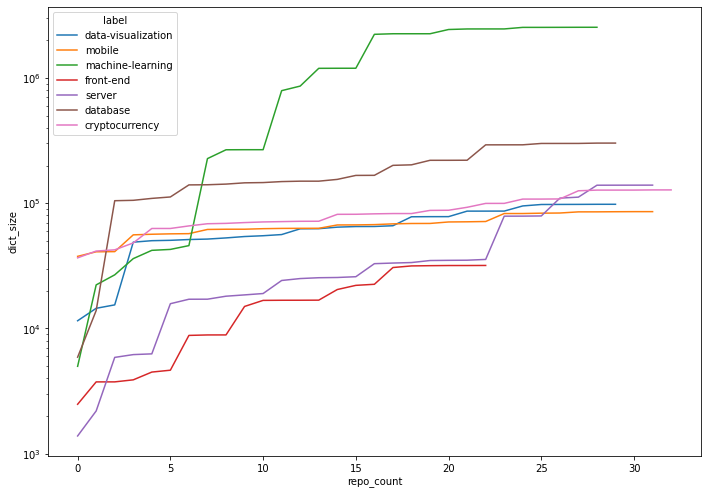
\includegraphics[width=\linewidth]{vocabulary.png}
  \caption{Size of the vocabulary for number of \textit{GitHub} projects that are tagged with the same concept. Each curve flattens after a few projects are added to the set of projects, \eg for the concept \enquote{machine learning} 16 projects are required, and for the concept \enquote{database} only 2 projects are required.}
  \label{KM:Fig:Vocabulary}
\end{figure}

\paragraph{Use Cases \& Requirements}
\label{KM:SubSec:UseCasesAndRequirements}
Our interactive visualization technique addresses two main use cases.

\begin{description}
\item[UC-1:] The proposed visualization should be able to support a project managers daily work in locating experts for general concepts among the developers.
It should facilitate the detection of developers that are active in a general concept, and it should also be able to relate developers to each other, \ie if a developer leaves a project.
\item[UC-2:] On a broader perspective our visualization should be able to monitor the distribution of knowledge across an entire IT organization in order to detect risks at an early stage.
\end{description}

\section{\uppercase{Related Work}}
\label{KM:Sec:RelatedWork}

\noindent Our work mainly extends ideas presented by Linstead \etal, who were the first to mine developer expertise using probabilistic topic models~\cite{linstead2007eclipseeeveloper,linstead09sourcerer}.
In particular, a developer's expertise in topics was determined using the \ac{ATM}, a variant of \ac{LDA}~\cite{rosen-zvi2004authors}, on  source code files.
In combination with \ac{MDS}, the similarity between the developers can be visualized as a two-dimensional scatter plot.

Saxena and Padanekar proposed an algorithm for mining and visualizing a developer's expertise in abstracts concepts~\cite{saxena2017know}.
By annotating a developers import statements with tags from Q\&A-forums, \eg \textit{Stack Overflow}, each developer was assigned a level-of-expertise in the concept.
Based on the underlying hierarchy of concepts, each developer was visualized using a treemap.

Greene and Fisher developed \textit{CVExplorer}, an approach for mining and visualizing technical skills for \textit{GitHub} users~\cite{greene2016cvexplorer}.
Their approach extracts the commit messages, the changed files, and the Readme files for each repository a user has contributed to.
By comparing the commit messages and the Readme files with a white list of skills, and extracting the programming language from the modified files, each developer is assigned a skill level.
The skills for each developer are displayed as an interactive tag cloud.

Kourtzanidis \etal trained the Microsoft Language Understanding Intelligent Service (LUIS) to identify expertise in two front-end frameworks and three .Net technologies~\cite{kourtzanidis2020reposkillminer}.
The authors developed a tool, named \textit{RepoSkillMiner}, which visually communicates a developer's profile using basic two-dimensional charts.

Other approaches for mining aspects of developer expertise include familiarity with source code~\cite{Fritz2014Degree}, libraries~\cite{Teyton2013Library}, or abstract concepts~\cite{teyton2014expertise}.

Skupin was the first to apply dimension reduction techniques for the task of displaying semantic relatedness between natural language documents~\cite{skupin2004worldofgeography}.
Applying Self-Organizing Maps on the \ac{BOW} of abstracts from publications results in a two-dimensional layout that was enriched using cartographic methods.

Kuhn \etal presented a similar method for the software visualization domain, to capture the \enquote{semantic} similarity between source code files, \ie files that implement a common semantic should be placed near each other~\cite{kuhn2008consistentlayout,kuhn2010software}.
Their layout is determined using \ac{LSI}, a non-probabilistic topic model~\cite{deerwester1990indexing}, together with \ac{MDS} on the natural language used in the source code files.

Atzberger \etal presented \textit{Software Forest}, a 2.5D visualization, whose layout originates from \ac{LDA} and \ac{MDS} applied on the comments and identifier names found in source code files~\cite{atzberger2021softwareforest}.
By placing 3D glyphs, \eg trees, on the plane numerical attributes associated to a source code file can be displayed.
Their layout approach was later applied to the 3D case, leading to a visualization of development activities in source code using a Galaxy metaphor~\cite{atzberger2021-softwaregalaxy}.

\section{\uppercase{Mining Developer Expertise from Source Code Activities}}
\label{KM:Sec:ConceptExpertise}

\begin{table*}[t]
    \centering
    \caption{Most relevant terms $(\lambda = 0.6)$ for six exemplary concepts.}
    \label{tab:topics_LLDA}    
    \footnotesize    
	\setlength{\tabcolsep}{10.0pt}%
	\renewcommand{\arraystretch}{1.30}
    \begin{tabular}{c|c|c|c|c|c}
    \toprule
    \textbf{Machine Learning} & \textbf{Mobile} &
    \textbf{Cryptocurrency} & \textbf{Database} & \textbf{Server} & \textbf{Data Visualization}\\ \midrule
         th & android & fe & err & span & chart \\
         tensor & view & order & db & request & prop \\
         self & name & symbol & table & server & series \\
         cuda & com & crypto & test & test & axis \\
         input & get & binance & key & header & pixi \\
         model & param & price & name & http & gl \\
         license & conv & trade & value & rct & datum \\
         output & activity & wallet & opt & body & react \\
         layer & fpga & exchange & sql & response & point \\
         size & wishlist & block & error & message & style \\
         \hline
    \end{tabular}

\end{table*}

\noindent As discussed in \Cref{KM:SubSec:Data}, the vocabulary used in the commits is a strong indicator for a developer's fields of expertise.
This motivates the use of techniques from the \ac{NLP} domain for mining developer expertise.
One of the most widely used class of algorithms for mining software repositories are topic models~\cite{chen2016survey}.
In this section, we detail our approach on how we apply \ac{LDA}, a probabilistic topic model introduced by Blei \etal~\cite{blei2003latent}, and its variant \ac{LLDA}, proposed by Ramage \etal~\cite{ramage2009labeled}, for modelling a developer's expertise based on his source code activities.

\paragraph{Data Preprocessing}
\label{KM:SubSec:DataPreprocessing}

For each developer, we extract his commit history from the \ac{VCS} and store the entire set of added and deleted files in a single document.
Before applying the respective topic model, the vocabulary is required to be preprocessed to remove words that carry no meaning and to decrease the size of vocabulary.
We adopt the preprocessing steps proposed by Atzberger \etal \cite{atzberger2021softwareforest},\ie (1) we remove non-text symbols, \eg commas or semicolons, (2) we split words at delimiters and according to the Camel Case convention, (3) we remove stop words of the English language and keywords of the programming language, and (4) we lemmatize the vocabulary.

\noindent After the preprocessing is performed, we store each document in the \ac{BOW} format, thus neglecting the order of the single words and just storing their frequency.
From now on, when we refer to the commit history of developers, we always mean the preprocessed \ac{BOW}s.

\paragraph{Latent Dirichlet Allocation for Mining Developer Similarity}
\label{KM:SubSec:LDA}

Given a set of documents $\mathcal{C} = \{d_1, \dots, d_m\}$, the so-called \textsl{corpus}, the goal of a probabilistic topic model is to extract latent topics $\varphi_1, \dots, \varphi_K$ in the corpus by examining patterns of co-occurring words.
The number of topics $K$ is a hyperparameter of the model and needs to be set by the user initially.
The extracted topics are given as distributions over the vocabulary $\mathcal{V}$, which contains the terms from the corpus $\mathcal{C}$.
In most cases, the underlying \enquote{concept} of a topic can be derived from its most probable words~\cite{markovtsev2017topic}.
Moreover, topic models learn representations $\theta_1, \dots, \theta_m$ of the documents as distributions over the topics.
The distributions $\theta_1, \dots, \theta_m$ are therefore descriptions of the semantic structure of the document.

The core assumption of \ac{LDA} is that the corpus underlies a generative process, which is given by

\begin{enumerate}
    \item For each document $d$ in the corpus $\mathcal{C}$ choose a distribution over topics $\theta \sim \text{Dirichlet}(\alpha)$
    \item For each word $w$ in $d$
    \begin{enumerate}
        \item Choose a topic $z \sim \text{Multinomial}(\theta)$
        \item Choose the word $w$ according to the probability $p(w \vert z, \beta)$
    \end{enumerate}
\end{enumerate}

By associating each developer with its respective commit history, the application of \ac{LDA} extracts the hidden concepts, as well as describes each developer as a distribution over topics, \ie each developer is described as a high-dimensional vector of dimension $K$.

\paragraph{Locating Concept Expertise using Labeled LDA}
\label{KH:SubSec:LLDA}

Direct application of \ac{LDA} does not provide labels for the extracted topics.
Especially when applied on source code files from a single project, the interpretation of topics requires an in-depth knowledge about a project~\cite{linstead09sourcerer}.
Pure \ac{LDA} is therefore not applicable for locating expertise among developers in general concepts, \eg \textit{Machine Learning}, \textit{Mobile}, \textit{Front-End}, or \textit{Cryptocurrency}.

\ac{LLDA}, a variant of \ac{LDA} proposed by Ramage \etal can be used to extract labeled topics~\cite{ramage2009labeled}.
Assuming that each document $d_1, \dots, d_m$ in the training corpus is provided with tags as meta information, each topic is associated with exactly one tag.
Vice versa a document can only have a non-zero value in a topic, when it is provided with the corresponding tag.
The idea behind our approach is to generate a corpus of labeled software projects, that serve as representatives for the general concepts.
\textit{GitHub Topics}\footnote{https://github.blog/2017-01-31-introducing-topics/} provide a tagging system for projects hosted on \textit{GitHub}.
Using the \textit{GitHub API} it is possible to select all projects that are tagged as examples for a general concept.
To extract the \enquote{real} software projects, we neglect all projects that are additionally equipped with tags from a white list that contains words like, \textit{awesome-list}, \textit{tutorial}, or \textit{interview}.
To ensure, that the project is actively maintained, we further filter all projects with less than 20 open or closed issues.
The remaining projects are sorted according their \textit{stars}\footnote{https://docs.github.com/en/get-started/exploring-projects-on-github/saving-repositories-with-stars} in decreasing order.
For example the first four elements of the list of projects for the concept \textit{machine-learning}, are \textit{tensorflow/tensorflow}, \textit{keras-team/keras}, \textit{pytorch/pytorch}, and \textit{scikit-learn/scikit-learn}.
To reduce the training time, we reduce the size of the corpus utilizing the second observation discussed in \Cref{KM:SubSec:Data}, \ie the size of the vocabulary for a concept flattens after a few projects.
We stop adding documents to a concept, when the vocabulary increases less than \SI{1}{\percent} within the last five projects.

After selecting the projects for our training corpus, we join each source code file of a project to a single document, undertake the preprocessing steps described in \Cref{KM:SubSec:DataPreprocessing} and store them as a \ac{BOW}.
The application of \ac{LLDA} then leads to a description of concepts of interest as distributions over the vocabulary.
However, not always the most probable words are the best indicators for a concept, \eg words that would occur in all projects very frequently would be assigned a high probability in all topics.
In order to increase the interpretability of each topic, we compute the relevance values for each term $w$ in each topic $k$ according to the formula
\begin{align}
    r(w,k \vert \lambda) = \lambda \cdot \log(\varphi_{w,k}) + (1 - \lambda) \log \Bigg( \dfrac{\varphi_{w,k}}{p_w} \Bigg),
\end{align}
where $\varphi_{w,k}$ means the probability of the word $w$ in topic $k$ and $p_w$ is the marginal probability of the word $w$ in the corpus~\cite{sievert2014ldavis}.
\Cref{tab:topics_LLDA} shows the most relevant terms, according to a balancing factor of $\lambda = 0.6$ for the concepts \textit{Machine Learning}, \textit{Mobile}, \textit{Cryptocurrency}, \textit{Database}, and \textit{Server}, and \textit{Data Visualization}.
The frequency of the 50 most relevant terms for each concept are counted in the commit history of each developer.
Based on the frequency, we assign a discrete skill level between one and five to each developer, according to his \SI{20}{\percent}-quantile, \ie a developer who belongs to the \SI{20}{\percent} of developers who most often use the relevant words is associated with skill level five.

\begin{figure*}[t] %
    \begin{tikzpicture}[figNS, spy using outlines = {style = spyRC, magnification = 1.8, size = 24mm}]
        \node[figRC, anchor = center](fig0) at (0,0)
            {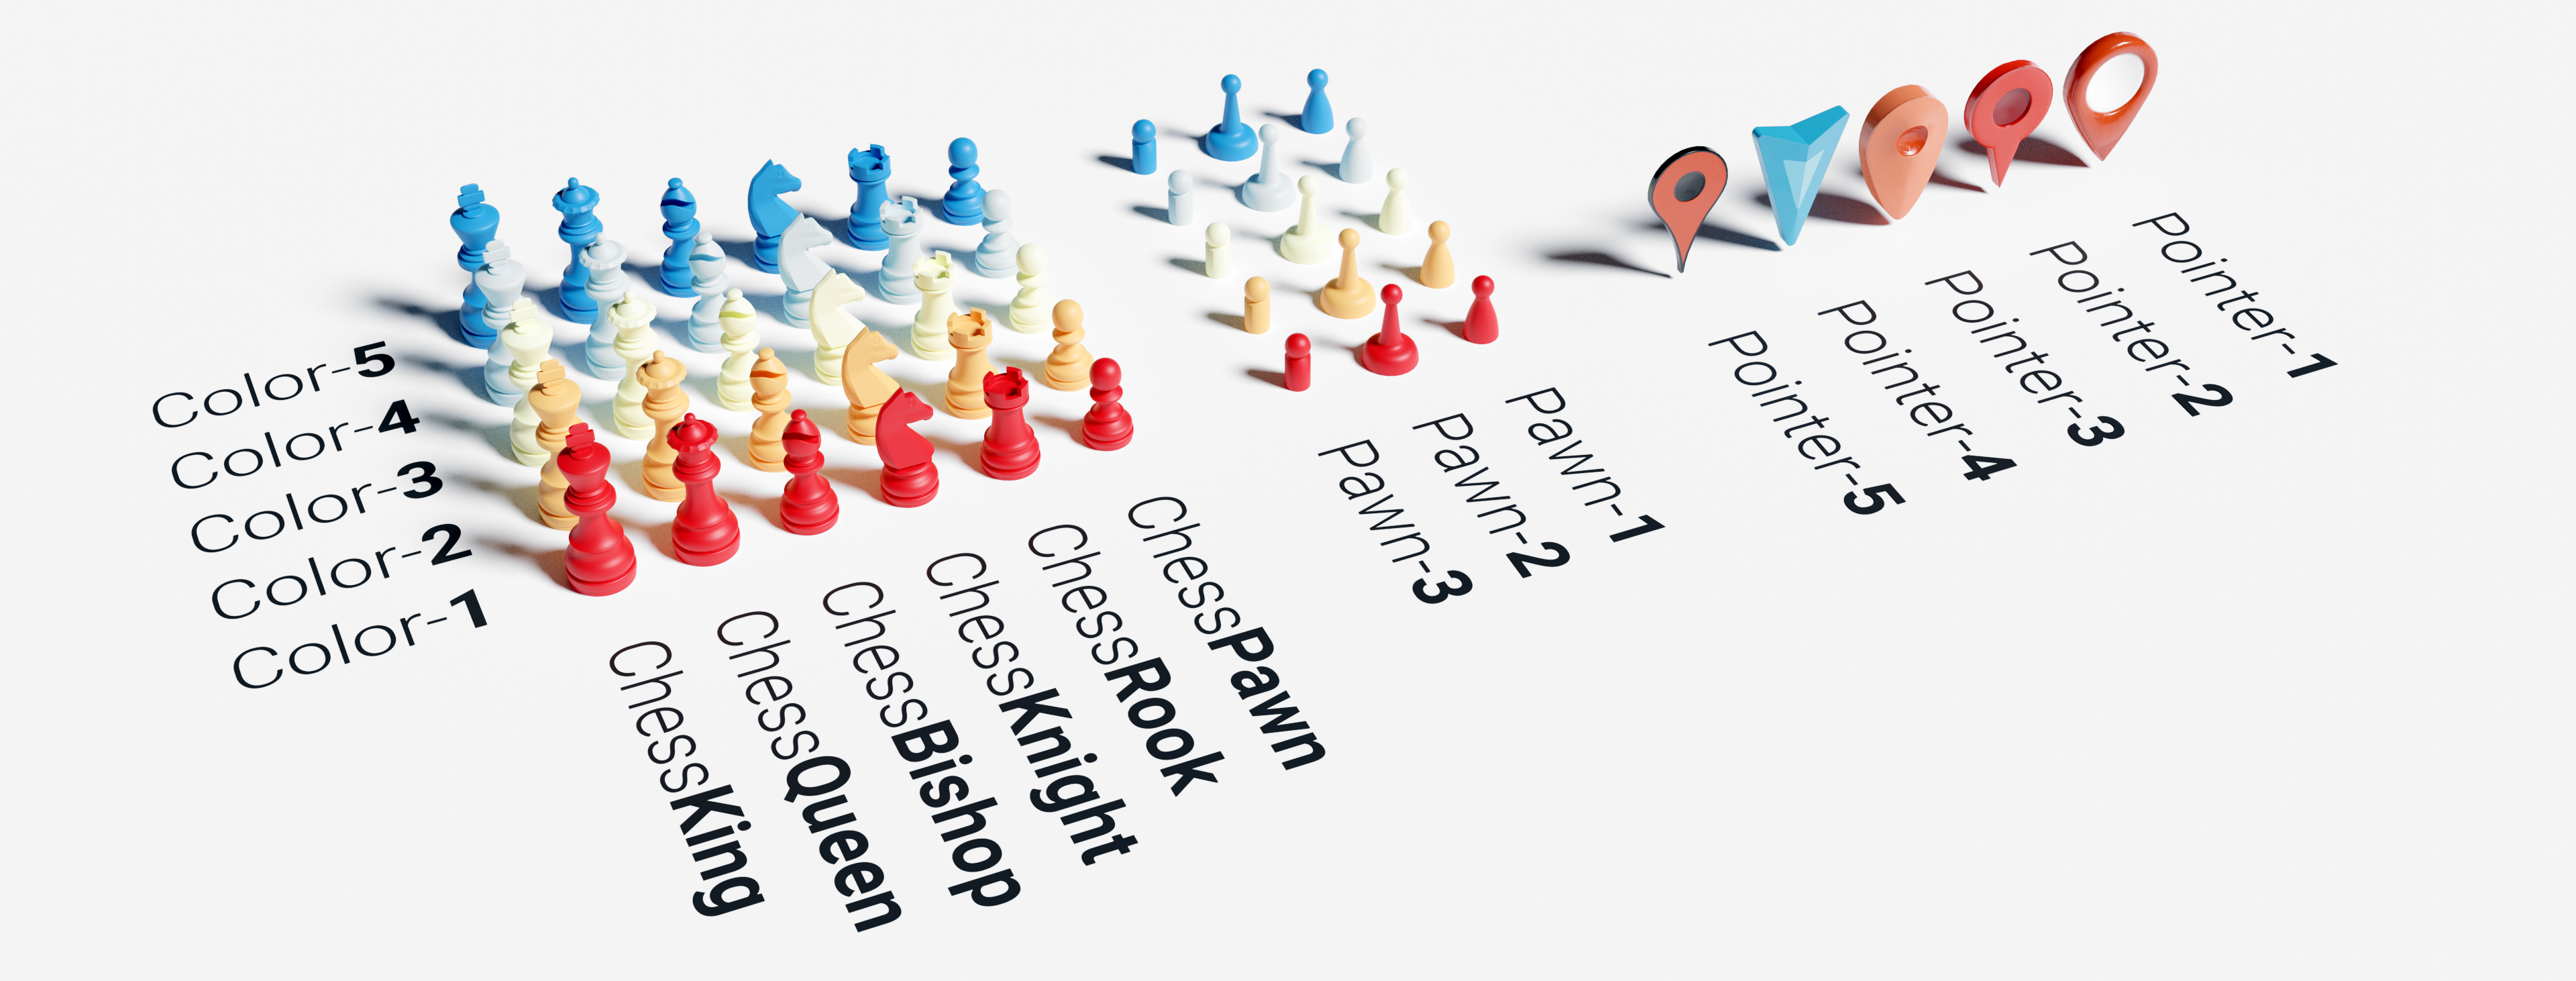
\includegraphics[width = \textwidth, trim = 0 0 0 0, clip]{figures/gltf-model-atlas-labeled-v2-trimmed-gamma}};
    \end{tikzpicture}
    \caption{Exemplary atlas of 3D glyphs for representing developers and topics. This atlas uses a diverging 5-color scale for the chess figures and the boardgame pawns. The pointers can be used as landmarks, e.g., for pinpointing the locations of topics.}
    \label{KM:Fig:3dglyphs}
\end{figure*}

\section{\uppercase{Visualization Approach}}
\label{KM:Sec:VisualizationApproach}

\noindent Our visualization comprise two main parts: (1) the computation of the layout, displaying semantic relatedness between developers, and (2) the mapping of data to the geometric representations for each developer.
The resulting visualization can be categorized as $\mathcal{A}^3 \oplus \mathcal{R}^2$, \ie three-dimensional graphical primitives on a two-dimensional reference space \cite{duebel2014-2d3drepresentation}.
By adding interaction techniques, \eg Zoom, Rotation, and Picking, the user is enabled to explore the map as part of the knowledge mining process.

\paragraph{Layout Technique}
\label{KH:SubSec:Layout}

The objective of our layout computation, is to map the similarity of two developers by Euclidean distance on a two-dimensional reference plane.
Although the developers can be compared with each other on the basis of their topic distributions using the Jensen-Shannon distance, the assumption is implicitly made here that all topics are orthogonal to each other, even though topics are themselves distributions over the vocabulary.
The layout approach by Atzberger \etal circumvents this problem.
In detail, given the latent topics $\varphi_1, \dots, \varphi_K$ from the corpus of commit histories, their dissimilarities can be measured using the Jensen-Shannon divergence and stored in a square matrix $\Lambda$.
\ac{MDS} applied on the dissimilarity-matrix $\Lambda$ results in $K$ points $\bar{\varphi}_1, \dots, \bar{\varphi}_K \in \mathbb{R}^2$, such that the Euclidean distance between two points $\bar{\varphi}_i$ and $\bar{\varphi}_j$ represents the entry $\Lambda_{ij}$ in the dissimilarity matrix~\cite{cox2008multidimensional}.
The position for a developer, described as distribution $\theta = \Big( \theta^{(1)}, \dots, \theta^{(K)} \Big)$ over the topics, is aggregated as a convex linear combination
\begin{align}
    \bar{\theta} = \sum \limits_{i=1}^{K} \theta^{(i)} \bar{\varphi}_i.
\end{align}

\begin{figure}[b] %
    \begin{tikzpicture}[figNS, spy using outlines = {style = spyRC, magnification = 1.8, size = 24mm}]
        \node[figRC, anchor = center](fig0) at (0,0)
            {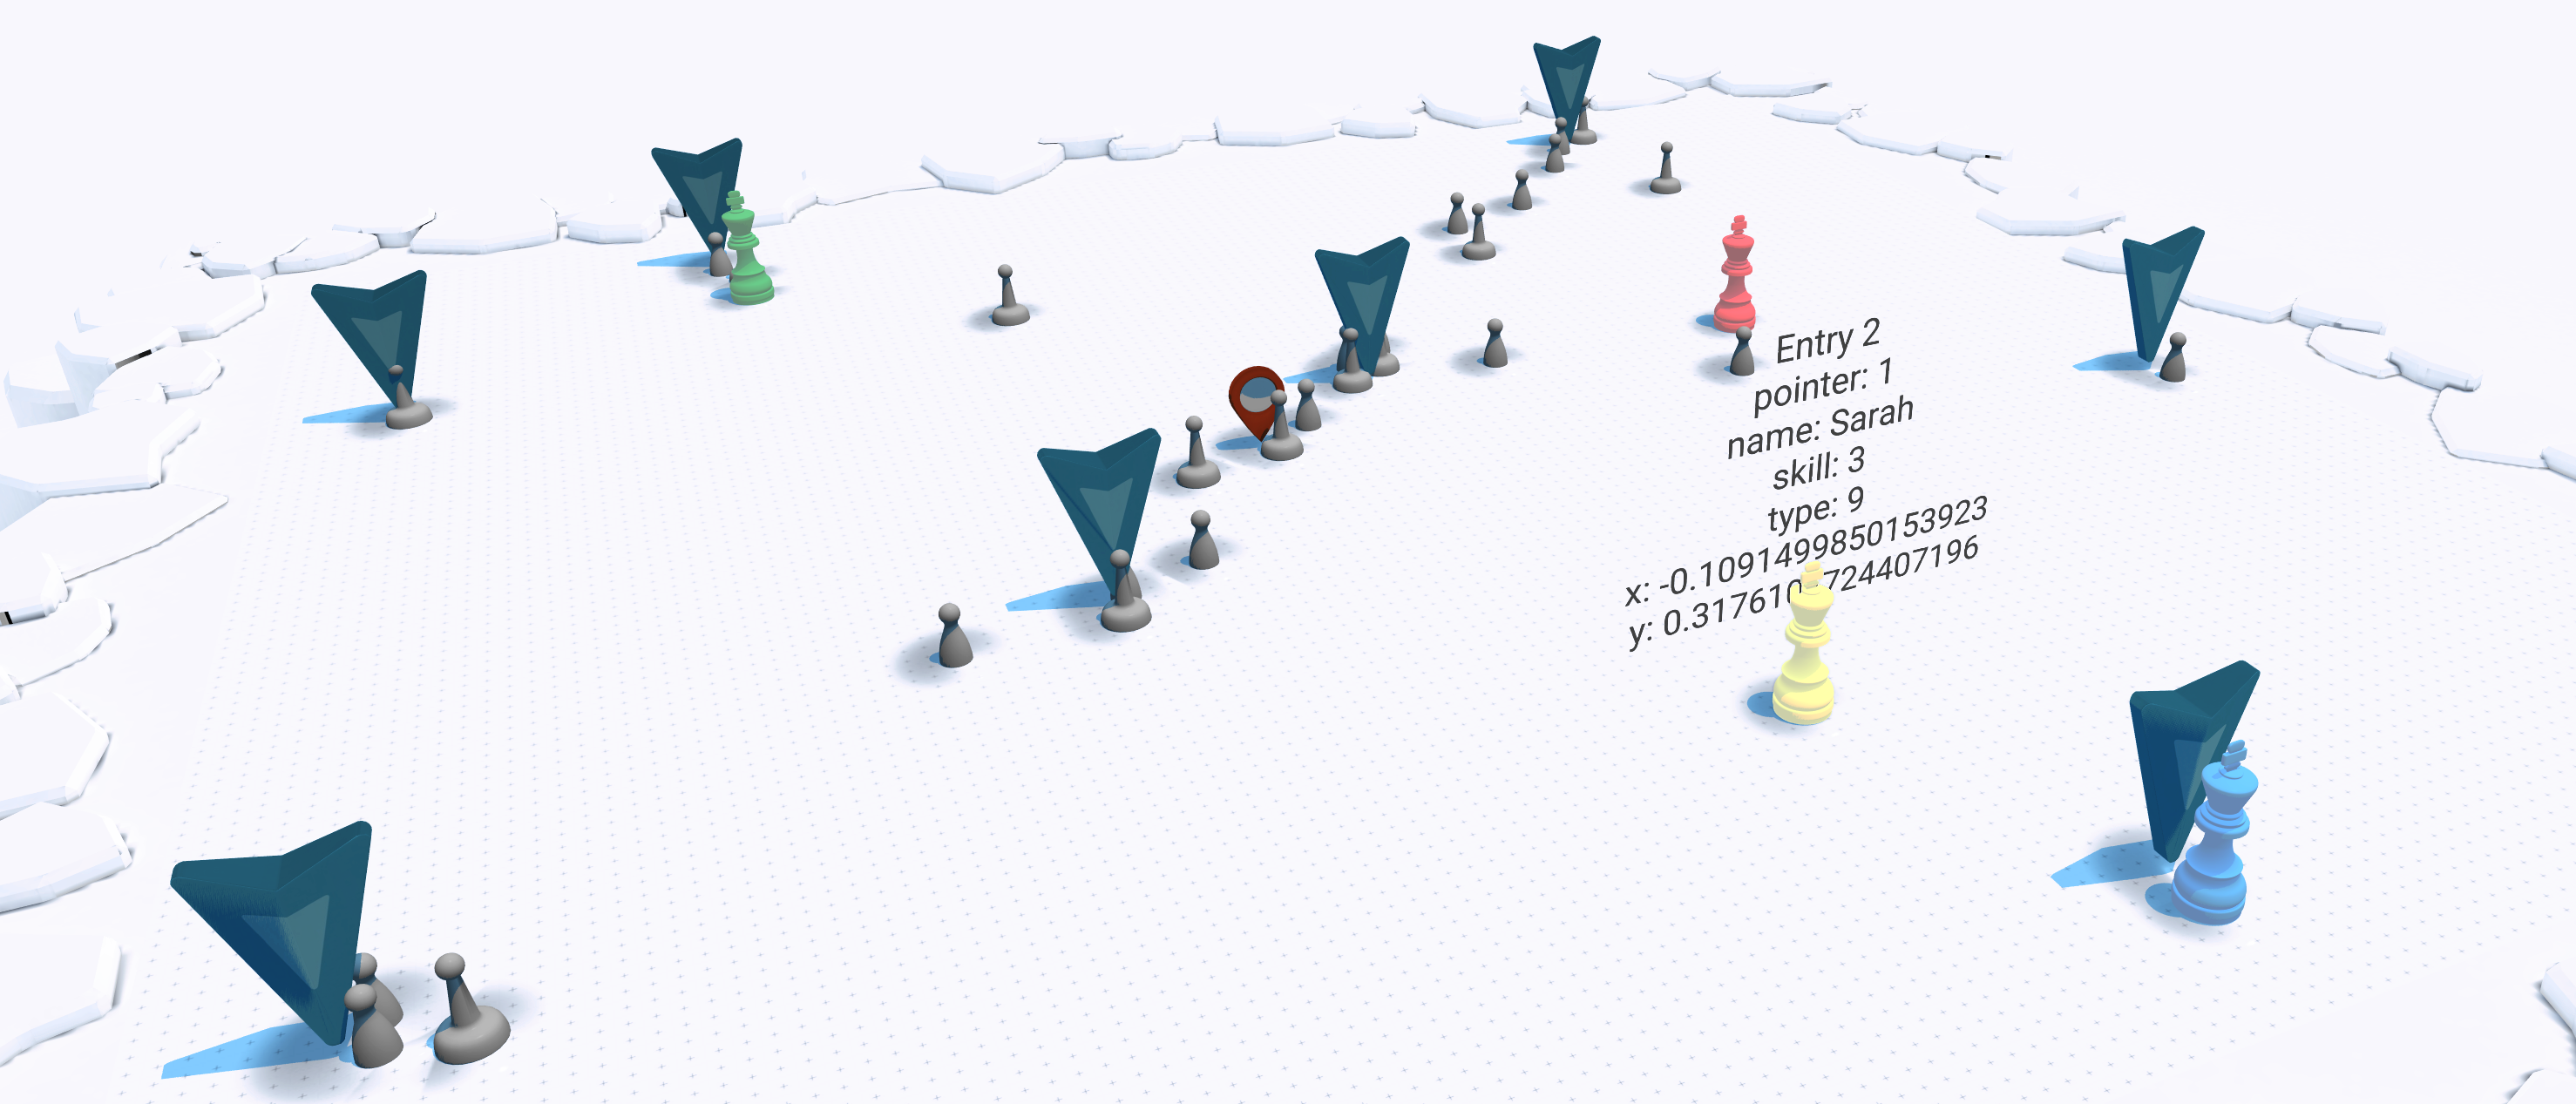
\includegraphics[width = \linewidth, trim = 0 0 0 0, clip]{figures/knowhowmap-gloperate-v1-trimmed-gamma}};
         sub-captions/labels:
        \node[above right = 0 of fig0, labelNE](lab0){(a)~Blue Print};
         spies:
        \spy on ($(fig0.center)+(+15mm, +1.25mm)$) in node at ($(fig0.north)+(-22mm,-2mm)$);
    \end{tikzpicture}
    \caption{\textit{KnowhowMap} showing a tooltip for a developer to display its position and other attributes.}
    \label{KM:Fig:Tooltip}
\end{figure}

\paragraph{Visual Mapping}
\label{KM:SubSec:Mapping}

Our map-related representation shows two types of objects, topics and developers.
We decided to use modelled 3D glyphs from \textit{SketchFab}\footnote{\url{https://sketchfab.com/}} for their representation, as shown in \Cref{KM:Fig:3dglyphs}.
Our system allows the user to manually choose a visual mapping supporting his task.

Topics are presented as pointers, reminding on geographical landmarks.
Their purpose is to locate experts in abstracts topics hidden in the source code, support navigating through the set of developers and help creating a mental map.
The only visual variable is given by the size and might be accessed for mapping the weight of the topic for the corpus.

Developers are depicted either using pawns or Chess figures.
Using a diverging color scheme of five colors, qualitative data can be mapped onto the visual attribute color~\cite{ware2019information}.
Furthermore, the type of figure, \eg \textit{Chess:King} or \textit{Chess:Knight}, can also be used for displaying qualitative information about a developer, \eg his rank within the software developing.
Another visual attribute is the height of each individual figure, which can be used for quantitative data attributes.
When we visualize the skill level of a developer, we always make use of the height of each individual glyph.

\paragraph{Implementation Aspects}
\label{KM:SubSec:Implementation}

Our data processing pipeline is written in the programming language \textit{Python}.
We use the lemmatizer provided by the library \textit{Spacy}\footnote{\url{https://spacy.io/api/lemmatizer}}.
We further use the \textit{nltk} package\footnote{\url{https://www.nltk.org/}} for accessing the stopwords of the English language. 
For training an \ac{LDA} model, we use \textit{Gensim}\footnote{\url{https://radimrehurek.com/gensim/}}.
The training corpus, consisting of \textit{GitHub} projects, required for training an \ac{LLDA} model is created using the \textit{GitHub V3 Rest API}.
We use the \ac{LLDA} implementation provided by the Python library \textit{Tomotopy}\footnote{\url{https://bab2min.github.io/tomotopy/v0.12.2/en/}}, which implements the algorithm according to the original paper of Ramage \etal \cite{ramage2009labeled}.

With respect to the visualization prototype, the glyphs are 3D models obtained from \textit{SketchFab}, that are further processed using \textit{Blender}.
Each model is associated with a description file (in JSON-format), that specifies the attributes of each object.
Our rendering component is based on a \textit{WebGL}-based point-plotter written in \textit{TypeScript}~\cite{wagner2020-scatterplot} that is able to process large data sets.
Further, the prototype supports various interaction techniques, \eg Zoom, Rotation, and Picking single glyphs.
Via hoovering over a glyph, the user can access additional information via a tooltip as shown in \Cref{KM:Fig:Tooltip}.
Using the open-source project \textit{webgl-operate}\footnote{\url{https://github.com/cginternals/webgl-operate}}, our 2.5D visualization is able to support labeling.

\section{\uppercase{Conclusions}}
\label{KM:Sec:Conclusions}

\noindent Mining developer expertise is of great interest for industrial software projects, as developers are the most important resource for any IT organization.
Existing approaches focus on mining selected aspects of developer expertise, but do not enable the user, \eg a project manager, to explore the distribution of skills and knowledge in an interactive way.

To address this problem, we propose a Visual Analytics framework for mining and visualizing developer expertise.
Each developer is modelled by applying \ac{LDA} on the commit history of all developers, thus leading to a mathematical formalization.
We further train an \ac{LLDA} model on a dynamically generated corpus of \textit{GitHub} projects to locate expertise in general concepts among developers.
The 2D layout of our visualization is derived from \ac{LDA} and \ac{MDS} and reflects the semantic similarity between developers and latent topics.
We choose 3D glyphs as graphical representation of developers and topics.
It is up to the user to choose a mapping between the data related to developer expertise and the visual variables of the glyphs, \eg color, size and shape.

However, our visualization allows different mappings and it is unclear which mapping is best-suited for each individual task.
There, the most important question, that needs to be addressed in future work, is the study of the effectiveness of our approach.
We plan to conduct a user study, by interviewing project managers of software projects from industry.
We are optimistic that real-world feedback could help to improve our visualization technique.

\section*{\uppercase{Acknowledgements}}
\label{sec:acknowledgements}
\noindent
We want to thank the anonymous reviewers for their valuable comments and suggestions to improve this article.
This work is part of the \enquote{Software-DNA} project, which is funded by the European Regional Development Fund (ERDF or EFRE in German) and the State of Brandenburg (ILB).
This work is part of the KMU project \enquote{KnowhowAnalyzer} (Förderkennzeichen 01IS20088B), which is funded by the German Ministry for Education and Research (Bundesministerium für Bildung und Forschung).

\bibliographystyle{apalike}
{\small
\bibliography{knowhow-map}}

\begin{acronym}
\acro{AST}{Abstract Syntax Tree}
\acro{ATM}{Author-Topic Model}
\acro{BMBF}{German Federal Ministry of Education and Research}
\acro{DTM}{Developer-Topic Model}
\acro{LDA}{Latent Dirichlet Allocation}
\acro{LSI}{Latent Semantic Indexing}
\acro{LOC}{Lines-of-Code}
\acro{NLP}{Natural Language Processing}
\acro{MBTI}{Myers-Briggs Type Indicator}
\acro{MDS}{Multidimensional Scaling}
\acro{MTM}{Multi-feature Topic Model}
\acro{SE}{Software Engineering}
\acro{BOW}{Bag-of-Words}
\acro{TTM}{Tag-Topic Model}
\acro{VCS}{Version Control System}
\acro{LLDA}{Labeled LDA}
\acro{OSS}{Open Source Software}
\acro{MDS}{Multidimensional Scaling}
\acro{LSI}{Latent Semantic Indexing}
\end{acronym}

\end{document}
